\documentclass[a4paper,ngerman,12pt]{scrartcl}

\usepackage[utf8]{inputenc}
%\usepackage[ansinew]{inputenc}

\usepackage[ngerman]{babel}

\usepackage{amsmath,amsthm,amssymb,mathtools,stmaryrd,color,graphicx}
\usepackage{setspace}
\usepackage{bussproofs}
\usepackage{array}
\usepackage{comment}
\usepackage{wrapfig}

\usepackage{enumitem}

\usepackage{units}

\usepackage[protrusion=true,expansion=true]{microtype}

\usepackage{lmodern}

\usepackage{hyperref}
\usepackage{cleveref}

\newcommand{\IR}{\mathbb{R}}
\newcommand{\IC}{\mathbb{C}}
\newcommand{\IZ}{\mathbb{Z}}
\newcommand{\IN}{\mathbb{N}}
\newcommand{\IQ}{\mathbb{Q}}

\setlength\parskip{\medskipamount}
\setlength\parindent{0pt}

\theoremstyle{definition}
\newtheorem{defn}{Definition}[]
\newtheorem{axiom}[defn]{Axiom}
\newtheorem{bsp}[defn]{Beispiel}

\RequirePackage{framed}
\newtheorem{aufg}{Aufgabe}
\definecolor{shadecolor}{rgb}{.96,.96,.96}
\newenvironment{aufgabe}[1][]
		{\begin{shaded}\vspace{-0.3cm}\begin{aufg}\emph{#1} \par\medskip}
		{\end{aufg}\vspace{-0.3cm}\end{shaded}}
\newtheorem{zaufg}{Zusatzaufgabe}
	
\newenvironment{spiel}[1][]{\begin{framed}\textbf{#1:}\\}{\end{framed}}


\theoremstyle{plain}
\newtheorem{prop}[defn]{Proposition}
\newtheorem{motto}[defn]{Motto}
\newtheorem{wunder}[defn]{Wunder}
\newtheorem{ueberlegung}[defn]{Überlegung}
\newtheorem{lemma}[defn]{Lemma}
\newtheorem{kor}[defn]{Korollar}
\newtheorem{hilfsaussage}[defn]{Hilfsaussage}
\newtheorem{satz}[defn]{Satz}
\newtheorem{frage}[defn]{Frage}

\theoremstyle{remark}
\newtheorem{bem}[defn]{Bemerkung}
\newtheorem{beob}[defn]{Beobachtung}

	
\newtheorem*{antwort}{Antwort}

%\newlength{\aufgabenskip}
%\setlength{\aufgabenskip}{1.4em}
%\newcounter{aufgabennummer}
%\newenvironment{aufgabe}[1]{
%	\addtocounter{aufgabennummer}{1}
%	\textbf{Aufgabe \theaufgabennummer.} \emph{#1} \par
%}{\vspace{\aufgabenskip}}

\clubpenalty=10000
\widowpenalty=10000
\displaywidowpenalty=10000

\setlength\unitlength{1cm}

\usepackage{tikz}
\usetikzlibrary{calc}
\usepackage{tkz-euclide}
\usepackage{adjustbox}
\usepackage{algorithm2e}
\usepackage{pgfplots}

\RequirePackage{geometry}
\geometry{textwidth=17.0cm,textheight=25cm,footskip=1.5cm}


\newcommand{\kante}[2]{#1{-}#2}
\newcommand{\edge}[3]{\draw[thick] (#1) --node[rectangle,fill=gray!10]{$#3$} (#2);}

\begin{document}
	
\begin{picture}(0,0)
\put(0,-0.5){%
	
\includegraphics[scale=0.1]{logo-ifm}
}
\put(14.0,-3.5){%
	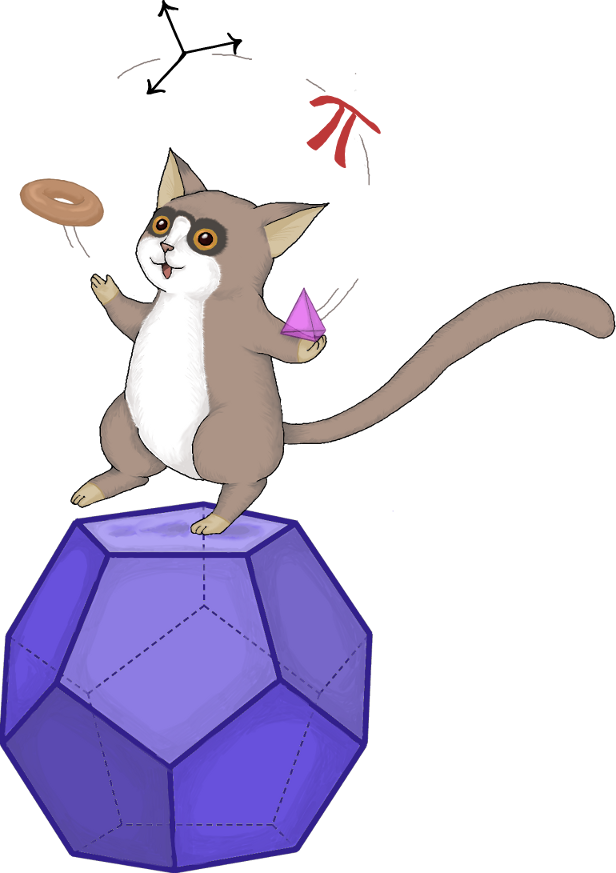
\includegraphics[scale=0.17]{cover}
}
\end{picture} 
	
\vspace{6em}

\begin{center}\Large{Mathe-Camp 2023}

\section*{Berechenbarkeit}\end{center}

\begin{aufg}
	Wir betrachten die folgenden Sprachen:
	\begin{itemize}
		\item Die deutsche Sprache (im Sinn von: Die Menge aller Wörter, die um Duden stehen)
		\item Die Menge aller Palindrome (Wörter, die von vorne und hinten gelesen gleich sind)
		\item Die Menge aller natürlichen Zahlen
		\item Die Menge aller Terme aus natürlichen Zahlen sowie den Rechenzeichen $+$ und $-$
		\item Die Menge aller solcher Terme, die $0$ ergeben
		\item Die Menge aller solcher Terme, die zusätzlich auch Klammern enthalten dürfen und korrekt geklammert sind
		\item Die Menge aller natürlichen Zahlen in einer festen Menge $S \subseteq \IN$
		\item Die Menge aller Computerprogramme (in einer fest gewählten Programmiersprache, z.B. Python)
		\item Die Menge aller terminierenden Computerprogramme
	\end{itemize}
	Überlege dir jeweils, was ein geeignetes Alphabet für diese Sprachen ist.
	
	Was denkst du: Welche dieser Sprachen ist entscheidbar?
\end{aufg}

\section{Endliche Automaten}

\begin{aufg}
	Welche der folgenden Sprachen über dem Alphabet $\{a,b,c\}$ kann von einem endlichen Automaten entschieden werden?
	\begin{itemize}
		\item Alle Wörter, die mit $a$ beginnen und mindestens ein $b$ enthalten.
		\item Alle Wörter, die nicht mit $c$ enden.
		\item Alle Wörter, die mit $aa$ beginnen und mit $b$ enden.
		\item Alle Wörter, die genau zwei $b$ enthalten.
		\item Alle Wörter, die eine durch $3$ teilbare Anzahl an $a$ enthalten.
		\item Die Sprache $\{\epsilon,ab,aabb,aaabbb\}$.
		\item Die Sprache $\{a^kb^k | k \geq 0\}$.
	\end{itemize}
\end{aufg}

\begin{aufg}
	Zeige mit Hilfe des Pumping-Lemmas, dass es für folgende Sprachen keinen endlichen Automaten gibt:
	\begin{itemize}
		\item $\{a^kb^k | k \geq 0 \}$
		\item $\{a^mb^k | k \geq m \geq 0 \}$
		\item $\{a^mb^k | m \geq k \geq 0 \}$
		\item $\{a^{k^2} | k \geq 0 \}$
	\end{itemize}
\end{aufg}

\begin{zaufg}
	Untersuche, ob die folgenden beiden Sprachen von einem endlichen Automaten entschieden werden können:
	\begin{enumerate}[label=\alph*)]
		\item Die Sprache aller Wörter aus $a$ und $b$, in denen die Buchstabenfolge $ab$ und $ba$ gleich oft vorkommen.
		\item $S \coloneqq \{a^p | p \text{ Primzahl}\}$
		
		\textit{Hinweis:} Zahlen der Form $n!+2$ könnten hier hilfreich sein.		
	\end{enumerate}
\end{zaufg}

\begin{zaufg}
	Ein \emph{un}endlicher Automat ist ein Automat, der genauso funktioniert wie ein endlicher Automat, aber unendlich viele Zustände haben kann. Überlege dir, ob diese Automaten mächtiger sind als endliche Automaten. Gibt es Sprachen, die auch ein unendlicher Automat nicht entscheiden kann?
\end{zaufg}

\section{Abschlusseigenschaften}

\begin{zaufg}
	Wir betrachten die Sprache
		\[\{a^mb^kc^k | m,k \geq 1\} \cup \{b^mc^k | m,k \geq 0\}.\]
	Diese Sprache kann von keinem endlichen Automaten entschieden werden.
	\begin{enumerate}[label=\alph*)]
		\item Warum können wir das nicht mit Hilfe des Pumping-Lemmas zeigen?
		\item Verwende eine geeignete Abschlusseigenschaft um diese Aussage zu zeigen.
	\end{enumerate}
\end{zaufg}

\section{Nichtdeterministische endliche Automaten}


\section{Kellerautomaten}

\begin{aufg}
	Welche der folgenden Sprachen kann von einem Kellerautomaten entschieden werden?
	\begin{itemize}
		\item Alle Wörter über dem Alphabet $\{a,b\}$ die gleich viele $a$ und $b$ enthalten.
		\item Alle Palindrome über einem festen Alphabet.
		\item $\{a^kb^kc^k | k \geq 0\}$
		\item Die Menge aller Wörter über dem Alphabet $\{(,)\}$, die einer korrekten Klammerung entsprechen.
	\end{itemize}
\end{aufg}

\begin{aufg}
	Finde zwei Sprachen $S_1$ und $S_2$ mit folgender Eigenschaft: Es gibt Kellerautomaten, die $S_1$ und $S_2$ entscheiden, aber keinen Kellerautomaten, der $S_1 \cap S_2$ entscheidet.
\end{aufg}

\begin{zaufg}
	Wir betrachten die Sprache aller Wörter der Form $wcw$, wobei $w$ ein beliebiges Wort aus den Buchstaben $a$ und $b$ sein kann. Gibt es einen Kellerautomaten, der diese Sprache entscheidet?
\end{zaufg}

\section{Turingmaschinen}

\begin{aufg}
	Finde eine Turingmaschine, die die Sprache $\{wcw | w \in \{a,b\}^*\}$ entscheidet.
\end{aufg}

\begin{aufg}
	Finde eine Turingmaschine, die die Sprache $\{a^kb^kc^k | k \geq 0\}$ entscheidet.
\end{aufg}

\begin{zaufg}
	Eine Keller-Turingmaschine ist eine (Einband-)Turingmaschine, die zusätzlich einen Keller zur Verfügung hat (der genauso funktioniert wie bei einem Kellerautomaten).
	
	Zeige, dass eine Einband-Turingmaschinen alles können, was Keller-Turingmaschinen können.
\end{zaufg}

\begin{aufg}
	Finde eine Turingmaschine, die auf manchen Eingaben nie hält.
\end{aufg}

\begin{zaufg}
	Wir betrachten die Sprache aller Kodierungen von Turingmaschinen, die das Wort, das ihrer eigenen Kodierung entspricht, nicht akzeptieren.
	
	Zeige, dass diese Sprache unentscheidbar ist.
\end{zaufg}

\begin{zaufg}
	Da Turingmaschinen das Band auch beschreiben dürfen, kann man den Inhalt des Bandes am Ende der Berechnung auch als Ausgabe interpretieren. Wir können also auch Turingmaschinen bauen, die eine bestimmte Ausgabe haben.
	\begin{enumerate}[label=\alph*)]
		\item Konstruiere eine Turingmaschine, die als Eingabe eine Zahl in Binärdarstellung erhält und diese dann um eins erhöht.
		\item Konstruiere eine Turingmaschine, die zwei Zahlen (in Binärdarstellung) erhält und diese zusammen addiert.
	\end{enumerate}
	\textit{Hinweis:} Es macht die Beschreibung der Turingmaschinen evtl. einfacher, wenn du annimmst, dass sie mehrere Bänder haben. Du musst die Turingmaschine außerdem nicht zwangsläufig komplett formal angeben.
\end{zaufg}

\end{document}